\documentclass[12pt]{article}

\usepackage{graphicx} % pictures
\usepackage{multicol} %Make columns
\usepackage{multirow} %Make rows
\usepackage{amsmath} % Mathy things
\usepackage{gensymb} % Literally only need for degree symbol why 
\usepackage{amssymb}
\usepackage{sympytex} 
\usepackage{booktabs} % Pretty Tables
\usepackage{colortbl} % Might replace xcolor for table  coloring
\usepackage{array} % Tably stuff
\usepackage{longtable} 
\usepackage[margin=1in]{geometry} %Change margins
\usepackage{fancyhdr} 
\usepackage{tabu} 
\usepackage{tabularx} 
\usepackage{pdfpages} % include pdf
\usepackage{pgfplots}
\usepackage{pgfplotstable}
\usepackage[per-mode=symbol]{siunitx}
\usepackage{float}
\usepackage[labelfont=bf,textfont=small]{caption} %Makes captions look nice, will use in the future (maybe)
\usepackage[hidelinks]{hyperref}
\usepackage{tocloft}

\renewcommand{\figurename}{Fig.}
\def\cequationautorefname{Equation}%
\usepackage{hyperref}
\usepackage{listings}
\pagestyle{fancy}
\fancyhead{}
\fancyfoot{}
\rhead{\hfill\thepage}
\lhead{\projectDescriptionShort}
\lstset{%
    basicstyle={\scriptsize\ttfamily},
    inputpath=./lvsreps
    }

\definecolor{lightgray2}{gray}{0.9} % Color for table rows

\newcolumntype{x}[1]{>{\centering\arraybackslash}p{#1}} %center fixed with columns 
%Use x{''width''}
\newfloat{cequation}{H}{equ}
\floatname{cequation}{Equation}
\newcounter{NameOfTheNewCounter}
\newcommand{\startalign}{\setcounter{NameOfTheNewCounter}{\theequation+1}}
\newcommand{\equationset}[1]{% \equationset{<caption>}
\noindent\makebox[\linewidth]{Equations \theNameOfTheNewCounter-\theequation: \textbf{#1}}\bigskip}% Print caption
%allow align environment numbering
\newcounter{engineering}
\renewcommand{\theengineering}{\Alph{engineering}}
\newcommand\engineerthis[1]{\refstepcounter{engineering}\label{#1}\theengineering. }
\newcommand\numberthis{\addtocounter{equation}{1}\tag{\theequation}}
\newcommand\Vcc{\ensuremath{V_{cc}}}
\newcommand\sip{\texttt{SI}}
\newcommand\clk{\texttt{clk}}
\newcommand\ao{\texttt{AO}}
\newcommand\mm{~\si{\milli\meter}}
\newcommand{\kohm}[1]{#1~\si{\kilo\ohm}}
\newcommand{\khz}[1]{#1~\si{\kilo\hertz}}

\setlength{\parindent}{0pt}
\setlength{\parskip}{6pt}

\graphicspath{{images/}}
\pgfplotsset{compat=1.13}
\pgfplotstableset{%
    %every head row/.style={before row=\toprule,after row=\midrule},
    every last row/.style ={after row=\bottomrule},
    every even row/.style={before row={\rowcolor[gray]{0.9}}},
}
% The following should be changed to represent your personal information
\newcommand{\projectDescription}{A smart solution to automate and regulate \\the feeding of common household pets}
\newcommand{\projectTitle}{Automated Pet Feeder}
\newcommand{\yourname}{Matt Smith}
\newcommand{\myname}{Chris Ranc}
\newcommand{\anothername}{Shabab Siddiq}
\newcommand{\dateSubmitted}{November 7, 2017}
%\newcommand{\collab}{In Collaboration with teams from Northeastern University, Georgia Tech, and Virginia Tech}
\newcommand{\componentDescription}{Dispensing Unit: Investigation into the physical design of the food dispensing unit.}
\newcommand{\projectDescriptionShort}{Dispensing Unit}


\setcounter{secnumdepth}{0} % Remove section numbering

\begin{document}
    
\thispagestyle{empty}
    \vspace*{2.5cm} 
    \begin{center}
        \LARGE
        \textbf{\projectTitle}

        \Large
        \projectDescription

    \vspace*{2.5cm} 
        \large
        \textbf{CMPE 495 Independent Risk Investigation}

        \componentDescription
    \end{center}
    
    \vspace*{2cm}
    
    \begin{multicols}{2}
        \phantom{LaTeX doesn't like empty columns} % Phantom will take up that much space, but not actually appear
        \columnbreak{}
        \begin{raggedright}
            
        Name: \yourname\\
        Team Members: \myname\
        \phantom{Team Members:} \anothername\\
        Submitted: \dateSubmitted\\
        \vspace{\baselineskip}
        \end{raggedright}
    \end{multicols}
\newpage
%
% TOC
%
\renewcommand{\cftaftertoctitle}{\thispagestyle{empty}} 
\renewcommand\cftsecleader{\cftdotfill{\cftdotsep}}
\tableofcontents
\newpage

\section{Overview}
%Brief textual description of the role of this high-risk component in the overall project
As a Computer Engineering project,physical design can carry the most risk as it's outside of our curriculum.one extremely important aspect of a physical design that carries the most risk is the actual method of dispensing food. As a dispensing unit, the design must be able to hold several days worth of food and be able to dispense without jamming or crushing the food. This design needs to be free of obstructions that would restrict food flow as well. Since the food will be gravity fed, we will also need to ensure that the assembly is not too top heavy such that it’d fall over with little effort.  
 
\section{Risk specification}
Marketing requirements for the dispensing unit:

\begin{enumerate}
    \item\label{supply} The feeder should be able to hold a multi-day supply of food.
    \item\label{remote} Must be able to control portions
    \item\label{reliable} Must be reliable enough to leave unattendend.
\end{enumerate}
The relevant specifications can be found in \autoref{tab:specs}.

\begin{table}[H]
    \centering
    \caption{Engineering Specifications}
    \label{tab:specs}
    \begin{tabularx}{\linewidth}{cXX} \toprule
        Marketing Requirement(s) & Engineering Requirement & Justification \\ \midrule
        \ref{supply}             &  An automatic feeder should have a multi-day supply of food & In order to justify an automatic feeder, the user must not need to tend to the feeder often.\\
        \ref{remote}              & Portion control for the feeder must be reliable and reasonably precise. & In order for the feeder to suit the needs of a diverse group of pets, the portions need to be controllable to accommodate size and health restrictions. \\
        \ref{reliable}            & Dispensing mechanism must be reliable enough to not jam or crush food too often.& It’s important that the unit does not jam because it’s designed to be trusted to feed while the owner is away for a reasonable time. A jam could mean a day without being fed.\\
    \end{tabularx}
\end{table}
%Many of these specifications, such as \ref{elight}, do not appear directly connected to the power system, but must be kept in mind, as they make options such as more batteries infeasible.
%Mostly tables introduced and explained in text

    %– Needs (0–2 points)—numbered customer needs or marketing requirements related to
    %this risk, (i.e., a subset of the overall project needs)
    %– Engineering specifications (0–2 points)—numbered/lettered engineering specification
    %related to this risk, each related to needs by number, (i.e., a subset of the overall project
    %specifications).
    %– Analysis to justify engineering specifications (0–3 points)
\section{Risk investigation}
%Combination of textual explanation and tables
    %– Survey of existing systems/components and how they relate to this risk (0–5 points)
    %– Concepts considered and chosen (0–3 points)
    %– Rationale for choice(s), including analysis performed, (e.g., Pugh table) (0–4 points)
    In order to have a cohesive system, the container must taper into a hopper that then feeds into the chosen dispensing mechanism. This means the hopper must be designed around the dispensing mechanism. As this mechanism carries the responsibility of both reliably and precisely dispensing food, it will be the primary focus of this investigation. Many future aspects of the design will be dependent on how food is dispensed from the unit, making this the lynch pin in the design.

When beginning to design and search for solutions, it’s often a good idea to look at solutions that already exist on the market for inspiration as well as learning based on others’ past decisions, productive or otherwise. A very common consumer item that was designed to specifically dispense dry goods is the cereal dispenser. These are often seen in hotels to provide varying kinds of cereal to patrons. These devices are manually controlled by a knob in the front that rotates a four-paddle
assembly that allows cereal to fall into a “V” shaped area, then the assembly rotates to drop the cereal down into a bowl below. This is a very common design due to the simplicity and the use cases associated with it. This design is particularly good at dumping larger servings into the bowl with the goal of filling it, but does not provide much room for precise control. This design also has a tendency to bind while rotating and in turn, pulverizing the dry food caught up. An illustration of this
can be seen in Fig. \ref{figure:bind}  in the appendix. This is often solved by the intelligent human operator rotating the assembly in the reverse direction then back in the original direction to clear the bind. With the intelligent user being replaced by an electric motor, the possible binding risks long term reliability on the design.

Another possible method seen in other dry goods dispensers is the simple trap door design. This idea can take many forms and orientations to allow food to spill out. This design is also very simple to implement. Similar to the paddle-based design, this method has trouble with precise dispensing. Unlike the paddle-based design, binding is rarely an issue due to the nature of an opening and closing door. It is possible that the door used in conjunction with a secondary dispensing method would allow to reduce the force of food stacked above the mechanism and by relation, reduce or remove possible binding. This possibility will need to be investigated further as well.

A third design possibility is not often seen in the context of moving dry food but is very common in automation applications such as injection molding, where a precise amount of material must be fed and injected into a mold. This design uses a a screw embedded into a tube that would allow for food to fall into the tube and the screw would rotate and push it along. The screw would be installed on an axle that could be easily driven by a motor. Since the screw would only allow small amounts of
food to fall between threads and pushed forward by the screw rotating, thus advancing the food to the drop point. This allows for the speed and the amount of food dispensed to be controlled with a far greater amount of precision. The downside to the screw based dispenser mechanism is that great care will be involved in designing the screw and hopper, particularly the angle of attack on the threads and the taper of the hopper. Any sort of binding could be greatly mitigated with a proper design, compared to the nature of the paddle dispenser that has far less room for improvement compared to the screw design.

\textbf{Concepts considered and chosen:}

First and foremost, the final design should be able to reliably portion and control the output of the pet food. Due to this, the most important design decision will be based on the mechanism that controls this. From research into feed methods, the screw design beats out other considered methods by a long shot in it’s ability to portion food in a semi controlled resolution compared to how the paddles and doors mostly dump the food.

Another point to consider is the durability of the design. For the paddle design, if a bind is encountered, a greater amount of torque would be needed for the paddle to overcome the bind compared to the screw. The screw can also be designed in such a way that the binding point would be far smaller. Another property of the mitigated screw design is that with a shallow angle of attack on the screw allows for food to be pushed back into the next gap between threads rather than getting stuck right away. Overall, the screw design, while being the more difficult design, can do the job of the dispensing mechanism the best out of other possible designs.

\section{Risk mitigation design}
%Technical details of proposed design choice—textual explanation with many meaningful
%diagrams, (introduced and explained in text); should include input(s) and output(s) and
%should define any interfaces/protocols
    %– Overview (0–2 points)
    %– How it works (0–10 points)—include specifications for this component to enable the
    %overall project to meet its engineering specifications, (which were presented in Section
    %II)
    %– Why this design mitigates, (i.e., eliminates or minimizes), risk (0–10 points)
    %– Overall risk subsystem diagrams (0–5 points)
    %– Detailed design (0–5 points)
        %· Circuits and assemblies, of any hardware components
            %o Circuit schematics
            %o Sensor types and placement
            %o Actuators
            %o Other components
            %o Interface(s) to other project components
            %o State diagrams, flowcharts, system models, etc.
        %· User interface and controls, of any software components
            %o State diagrams, flowcharts, system models, etc.
    %– Intellectual property (0–3 points)—results of patent search for design of proposed risk
    %solution
The most important aspect of the design being considered is the ability to portion food. Therefore the best choice for the dispensing mechanism is the feed screw design. With this choice the remainder of the dispenser can be designed around it. The overall design will be a vertical, gravity fed container to act as a hopper to feed into the feed screw. The feed screw will be held in a well fitting tube with a large enough tolerance allow dust past the edges. The tube under the hopper will be cut to allow food to enter and the end will be open to allow for the food to fall. The feed screw will be driven by a stepper motor to allow for precise control of the feed screw rotation. This will be constructed on an elevated base to allow for food to fall into the bowl.

The first focus of this design will be in the feed screw itself. A feed screw is a common design that is used in many applications including material extractions. It is very similar to a drill or auger in most ways except in that the feed screw remains stationary while augers or drills move. Since feed screws are relatively common of a design, it can be easy to find many examples online. For the purpose of a prototype and the lack of considerable modeling experience, open source designs will be
used as a jumping off point towards creating a working prototype. One particular design found provided the same service as this project, albeit far more simple and static in configuration. This design used a 3d printed auger within a PVC tube and fed by a plastic container. This 3D auger design can be modified to fit the scale of this design and be made to fit the motor of our choice. A 3D rendering of this design can be seen in Fig. \ref{figure:feed_screw}. This source project can be found in the appendix. 

Using this feed screw/auger design. Material must be selected for the outer tube. The original application called for a 1.5’’ female PVC T coupling. Since The inner diameter of this fitting is the outer diameter of standard PVC, the design will likely need to be modified to fit a standard sized piece of tubing. It would be beneficial to use a standard size pipe with a smooth interior to reduce and mitigate any possible binding that could be caused by a rough surface. PVC is also commonly used in water and food applications, making it a safe choice to use with food. It will still be important to have clean cuts and wash after working on it to ensure nothing could get into the animals food. 

In order to drive this feed screw, an electric motor with both feedback and continuous rotation will be
needed. A simple DC motor does not have the ability to know its rotational position and would not be a good
choice for driving something where you need fine control. A servo can be aware of position, but a continuous
servo loses that ability and is just a geared motor. A stepper motor can have fine grain control over
movement with the ability to rotate continuously in a single direction. The torque requirements of the
stepper motor is currently unknown, therefore specific decisions on motors and belt/pulley configurations are
currently unknown as well. What is known is that additional electronics will be needed to drive a stepper
motor using a micro controller. This will be a consideration for later in the design and is not within the
scope of this investigation. 

Finally, the hopper/food container can be made from durable acrylic panels. These panels can be cut to construct a proper taper at the bottom of the hopper to ensure smooth feeding.  The acrylic can be constructed via screws and pre-drilled holes, combined with a glue to seal it. This will result in a strong and safe container for an animal’s food to be held. A cover can be constructed in the same fashion to prevent foreign objects from falling in. 

 With proper clearances, this design will be able to avoid most binding while being powerful enough to push the food. The feeder screw allows for fine control due to how it releases small amounts of food per revolution. With a smooth outer tube and a correct blade angle, binding should be rare. This setup allows for food to be filled high in the hopper, supporting a multi-day food supply. 

%<risk subsystem diagrams>

%<Detailed Design>

In searching for patents of a similar design, one patent, US 6401657 B1, was found to be similar but not nearly identical in form or purpose. This device uses a very common auger feed delivery system but the bowl is integrated in the unit. It does not extend to the extended functionality of the design. 

\section{Parts List}
%List of parts for proposed risk mitigation design.
    %– Part description (with name and number, if applicable)
    %– Cost—(standard purchase price of component)
    %– Your cost—(your cost for component; could be $0 if you already own)
    %– Availability—(vendor information, including lead time from order placement to delivery)
    At the current state of the design, the parts list is still uncertain. The availability of the 3D printed
    components is certain but the size and quality of the print makes it difficult to estimate costs. 
    The second point to consider is determining the best place to order may change in time so the "our cost" 
    will be left blank until specific components are finalized.
    \begin{table}[h]
\caption{Parts List} % title of Table
\centering % used for centering table
\begin{tabular}{c c c c} % centered columns (4 columns)
\hline\hline %inserts double horizontal lines
    Part & Cost & Our Cost & Availability \\ % inserts table
%heading
\hline % inserts single horizontal line
    3D Printed Feed Screw & TBD& & RIT Printers \\
    3D Printed base & TBD& & RIT Printers\\
    misc. 3D printed fittings & TBD& & RIT Printers\\
    Stepper motor & \$15-20 & & Available from amazon \\
    Stepper motor driver & \$5-15 & & available from amazon \\
    Acrylic sheet & \$5-10 & & available from Home Depot \\
    misc fasteners & TBD & & available local or online. \\

    \hline %inserts single line
\end{tabular}
\label{table:bom} % is used to refer this table in the text
\end{table}
\section{Testing strategy}
%Plan for verification of proper component/subsystem operation within the project’s
%particular operating environment. The plan should include what will be measured/tested
%along with an estimate of when. (Notes: 1. manufacturer’s performance specifications are
%often unachievable in practice, [e.g., new car mileage estimates]; 2. testing sooner is much
%better than later— whether this high-risk component will perform adequately in the overall
%project system needs to be determined as early as possible.)
Initial testing will consist of verification of the main functionality. The feeder dispenser should be able to reliably dispense food under it’s own power in small enough increments that would allow for proper portion control. Once the mechanism is functional alone, it can then be integrated into any driving logic from installed micro-controllers. Paired with the micro-controller, automatic feeding will be tested with several refills to ensure functionality. Within these tests, portions will be weighed and recorded to ensure consistent portions. If at one point this fails to be reliable, certain aspects of the design may need to be revisited. As hardware is the most difficult to make rapid changes to, much care will go into the design and functionality will be checked as early in the revision as reasonably possible.
\section{Uncertainties}
%Any remaining doubts or questions about using or testing this component/subsystem—any
%concerns the author or other team members have about this aspect of the project.
As this area of the design is outside the standard Computer Engineering curriculum, none of the team members are particularly skilled in modeling or mechanical design. This means that we will need to do a considerable amount of self learning and outside consultation to persons of distinguishable skill in the area. However, the scope of this design is not too far outside the abilities of competent “maker” and is not an unreasonable task.


\pagebreak
\section{Appendices}
%Copies of (or links to) the manufacturer’s literature on the component/subsystem—
%especially technical specification(s) and application notes.


\begin{figure}[H]
\centering
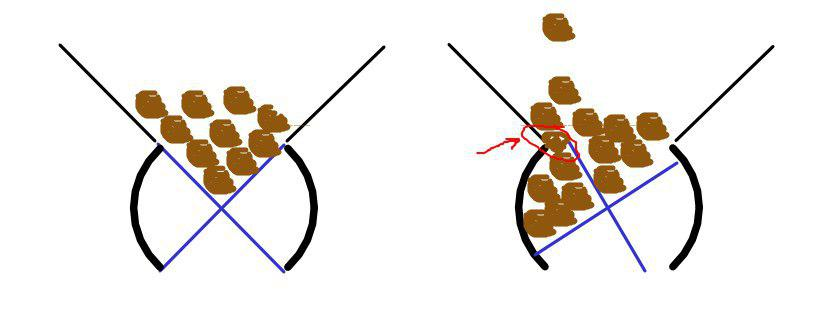
\includegraphics[width=1\textwidth]{bind}
\caption{Illlustration of food bind}
\label{figure:bind}
\end{figure}

\begin{figure}[H]
\centering
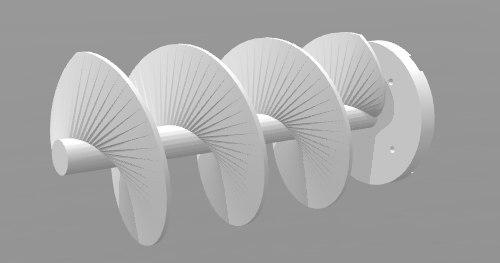
\includegraphics[width=.75\textwidth]{feed_screw}
\caption{3D model of feed screw base design}
\label{figure:feed_screw}
\end{figure}
\textbf{Sources:}

\textbf{Auger Based Cat Feeder- Thingverse:} https://www.thingiverse.com/thing:27854

\textbf{Possible stepper driver:} https://www.banggood.com/3Pcs-3D-Printer-A4988-Reprap-Stepping-Stepper-Step-Motor-Driver-Module-p-967057.html?rmmds=search&cur_warehouse=CN

\textbf{Possible stepper motor:} https://www.banggood.com/28YBJ-48-DC-5V-4-Phase-5-Wire-Stepper-Motor-With-ULN2003-Driver-Board-p-74397.html?rmmds=search&cur_warehouse=CN

\textbf{Patent found that is similar in design:} https://www.google.com/patents/US6401657


\end{document}
